\documentclass[serif,utf8]{beamer}
%russification
\usepackage[utf8]{inputenc}
\usepackage[russian]{babel}
%math mode
\usepackage{amssymb}
\usepackage{euscript}
\usepackage{amsmath}
\usepackage{amstext}
\usepackage{textcomp}
\usepackage{graphicx}
\usepackage{fancybox}
\usepackage{wrapfig}
\usepackage{multicol}
\usepackage{multirow}
%\usepackage[final]{graphicx}
\graphicspath{{image/}}

\usepackage{floatflt}
%\usepackage{pst-plot}
%theme
\usetheme{Copenhagen}

\usecolortheme{seahorse}

\setbeamersize{text margin left = 1.0 cm}
\setbeamersize{text margin right = 1.0 cm}

\setbeamertemplate{caption}[numbered]


\newtheorem{mydef}{Определение}

\begin{document}

%\setbeamercolor{block body}{BG=green}

\institute{МОСКОВСКИЙ ГОСУДАРСТВЕННЫЙ УНИВЕРСИТЕТ ИМ. М.В. ЛОМОНОСОВА \\ %
	ФАКУЛЬТЕТ ВЫЧИСЛИТЕЛЬНОЙ МАТЕМАТИКИ И КИБЕРНЕТИКИ \\ %
	КАФЕДРА МАТЕМАТИЧЕСКОЙ КИБЕРНЕТИКИ }
\title[Восстановление частичных СФЭ]{Исследование методов восстановления частично заданных схем из функциональных элементов}
\author[Трубицын Ю. А.]{Трубицын Юрий Алексеевич}
\date{Москва, 2017}
\titlegraphic{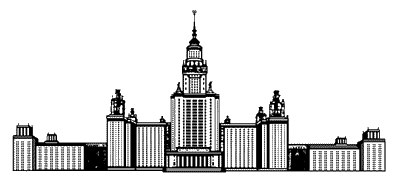
\includegraphics[ scale=0.2]{msu2.jpg}}


\begin{frame}
\maketitle
\end{frame}


\begin{frame}{Постановка задачи}
\begin{enumerate}
    \setbeamertemplate{enumerate items}[default]
	\item Выделить набор признаков СФЭ, которые будут использоваться для решения задачи распознавания, а также реализовать и протестировать алгоритмы вычисления признаков СФЭ;
	\item Построить регрессионную модель;
	\item Протестировать построенную модель на примере класса мультиплексорных функций. 
\end{enumerate}

\end{frame}


\begin{frame}{Исследование методов восстановления частично заданных схем из функциональных элементов}

Обозначим $X_{\scriptscriptstyle{\Sigma}} = \left\{ x_1, \dots, x_n\right\}$ -- множество входов схемы $\Sigma$, $Z_{\scriptscriptstyle{\Sigma}} = \left\{z_1, \dots , z_m\right\}$ -- множество выходов схемы $\Sigma$.\\
Введем также $X^{\ast} = \left\{ x^{\ast}_1, \dots, x^{\ast}_n, \dots \right\}$ -- счетный упорядоченный алфавит заходов удаленных контактов,
$Z^{\ast} = \left\{ z^{\ast}_1, \dots, z^{\ast}_n, \dots \right\}$ -- счетный упорядоченный алфавит исходов удаленных контактов.
\end{frame}

\begin{frame}{Исследование методов восстановления частично заданных схем из функциональных элементов}

\begin{mydef}
Частично заданной СФЭ (замаскированной СФЭ) $\Sigma$ будем называть такую схему $\Sigma^{'}$, которая получается путем удаления одного или нескольких ребер из исходной схемы $\Sigma$. При этом вершины, инцидентные удаленным ребрам помечаются некоторой переменной из множеств $X^{\ast}$ и $Z^{\ast}$ в зависимости от того, было ли ребро заходящим или исходящим.
\end{mydef}

\end{frame}

\begin{frame}{Исследование методов восстановления частично заданных схем из функциональных элементов}
Таким образом, формальная постановка задачи звучит так: реализовать алгоритмы, на вход которых подается частично заданная СФЭ, а выходом алгоритма должно быть решение о принадлежности объекта заданному классу.\par
Для тестирования алгоритма в качестве идентифицируемого класса взят класс схем, реализующих мультиплексорные функции.
\end{frame}

\begin{frame}{Исследование методов восстановления частично заданных схем из функциональных элементов}
Были выделены следующие признаки:
\begin{enumerate}
\item доля каждого возможного функционального элемента;
\item максимальная полустепень исхода вершин, нормированная на количество контактов в СФЭ;
\item максимальная полустепень захода вершин;
\item минимальная полустепень исхода/захода вершин;
\item средняя полустепень исхода/захода вершин;
\item средняя глубина, нормированная на максимальную глубину;
\item среднее количество присоединенных переменных, нормированное на общее количество переменных;
\end{enumerate}
\end{frame}

%\begin{frame}{Исследование методов восстановления частично заданных схем из функциональных элементов}
%\begin{mydef}
%Регрессионная модель $f(\mathbf{w},\mathbf{x})$ -- это параметрическое семейство функций, задающее отображение
%\begin{equation}
%f: W \times X \longrightarrow Y,
%\end{equation}
%где $\mathbf{w} \in W$ -- пространтсво параметров, $\mathbf{x} \in X$ -- пространство свободных переменных, Y -- пространство зависимых переменных.\\
%Модель является настроенной (обученной) когда зафиксированы её параметры, то есть модель задаёт отображение
%\begin{equation}
%f:X \longrightarrow Y
%\end{equation}
%для фиксированного значения $\bar{\mathbf{w}}$.
%\end{mydef}
%\end{frame}


%\begin{frame}{Исследование методов восстановления частично заданных схем из функциональных элементов}
%Пусть у нас множество $X$ представлено пространством всевозможных векторов,  размерность которых равна количеству признаков схем, выделенных для решения задачи распознавания.\par
%Множество $Y = \left\{ 0, 1 \right\}$.\par
%Если настроенная регрессионная модель возвращает 0, значит мы считаем, что некоторая СФЭ, набор признаков которой подавался на вход модели, не является мультиплексором. В случае, когда регрессионная модель возвращает 1, мы считаем, что некоторая СФЭ, набор признаков которой подавался на вход модели, наоборот, является мультиплексором.\par
%\end{frame}

\begin{frame}{Исследование методов восстановления частично заданных схем из функциональных элементов} 
Иcпользовались следующие алгоритмы машинного обучения:
\small{\begin{itemize}
\item метод опорных векторов (поиск разделяющей гиперплоскости с максимальным зазором в этом пространстве);
\item метод ближайших соседей (простейший метрический классификатор, основанный на оценивании сходства объектов; классифицируемый объект относится к тому классу, которому принадлежат ближайшие к нему объекты обучающей выборки.);
\item случайный лес (алгоритм машинного обучения, заключающийся в использовании комитета (ансамбля) решающих деревьев);
\item логистическая регрессия (метод построения линейного классификатора, позволяющий оценивать апостериорные вероятности принадлежности объектов классам).
\end{itemize}
}
\end{frame}

\begin{frame}{Исследование методов восстановления частично заданных схем из функциональных элементов}
Тестирование построенной модели проводилось на классе мультиплексорных функций.\\
Обучающая выборка состояла из схем следующего вида:
\begin{itemize}
\item Мультиплексоров;
\item Схем, <<близких>> к мультиплексорам (это мультиплексоры, на некоторые входы которых подаются мультиплексоры порядка 2, 3 или 4);
\item Случайные схемы, не являющиеся мультиплексорами.
\end{itemize}
Размер обучающей выборки равен примерно 600 схемам. Количество немультиплексорных и мультиплексорных схем равное.\par
\end{frame}

%\begin{frame}
%Для проверки точности полученных моделей использовался скользящий контроль.
%Скользящий контроль работает следующим образом:
%\begin{enumerate}
%\item Фиксируется некоторое множество разбиений исходной выборки; 
%\item Каждое из разбиений делится на две подвыборки: обучающую и контрольную; 
%\item Для каждого разбиения выполняется настройка алгоритма по обучающей подвыборке, затем оценивается его средняя ошибка на объектах контрольной подвыборки; 
%\item Оценкой скользящего контроля называется средняя по всем разбиениям величина ошибки на контрольных подвыборках.
%\end{enumerate}
%\end{frame}

\begin{frame}{Исследование методов восстановления частично заданных схем из функциональных элементов}
Для проверки точности полученных моделей использовался скользящий контроль.
На рис. \ref{picCV} показаны результаты скользящего контроля.\par
\begin{figure}[h!]
   \centering
   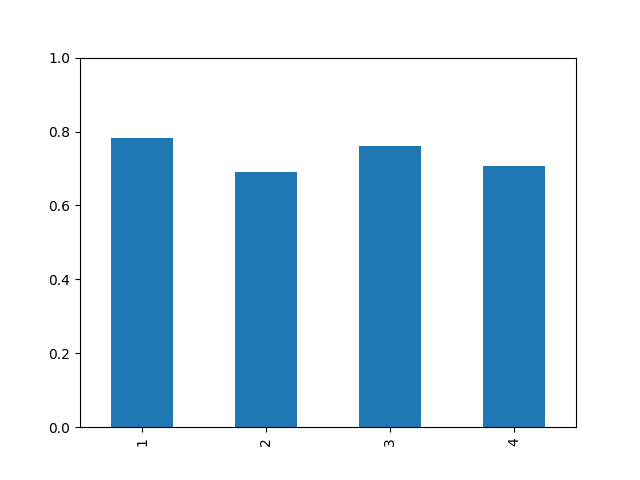
\includegraphics[width=0.5\linewidth]{cross_validation.png}
   \caption{\scriptsize{1 - случайный лес, 2 - метод ближайших соседей, 3 - логистическая регрессия, 4 - метод опорных векторов.}}
   \label{picCV}
\end{figure}
\end{frame}

\begin{frame}{Полученные результаты}
\scriptsize{
\begin{table}[h!]
\begin{tabular}[t]{|p{8em}|p{6em}|p{6em}|p{7em}|}
\hline 
	{Класс} & { Процент удаленных проводов} & { Случайный лес } & { Логистическая регрессия }\\
	{} & {  } & { } & { }\\
\hline
\hline
\hline
	\multirow{15}{*}{Мультиплексоры} 
		& {5\%}  & {0.997996} & {1.0}\\ \cline{2-4}
		& {10\%} & {0.997996} & {1.0}\\ \cline{2-4}
		& {15\%} & {0.997996} & {1.0}\\ \cline{2-4}
		& {20\%} & {0.998024} & {1.0}\\ \cline{2-4}
		& {25\%} & {0.997996} & {1.0}\\ \cline{2-4}
		& {30\%} & {0.998004} & {1.0}\\ \cline{2-4}
		& {35\%} & {0.998008} & {1.0}\\ \cline{2-4}
		& {40\%} & {0.998016} & {1.0}\\ \cline{2-4}
		& {45\%} & {0.998028} & {1.0}\\ \cline{2-4}
		& {50\%} & {0.998043} & {1.0}\\ \cline{2-4}
		& {55\%} & {0.998047} & {1.0}\\ \cline{2-4}
		& {60\%} & {0.998047} & {0.998054}\\ \cline{2-4}
		& {65\%} & {0.998058} & {0.997665}\\ \cline{2-4}
		& {70\%} & {0.998058} & {0.997005}\\ \cline{2-4}
		& {75\%} & {0.998095} & {0.996076}\\
\hline
\hline
	{Не мультиплексоры} & { - } & {0.994616} & {0.913862}\\ \cline{1-4}
\hline
\end{tabular}
\end{table}
}
\end{frame}


\begin{frame}{Полученные результаты}
\begin{enumerate}
\setbeamertemplate{enumerate items}[default]
\item Выделен набор признаков СФЭ, которые использовались для решения задачи распознавания, а также реализованы и протестированы алгоритмы вычисления признаков СФЭ;
\item Построена регрессионная модель;
\item Построенная модель протестирована на примере класса мультиплексорных функций. 
\end{enumerate}
\end{frame}

\begin{frame}
\maketitle
\end{frame}


\end{document}